% \documentclass{beamer}
% \usetheme{Boadilla}

% \usepackage[english,greek]{babel}
% % \usepackage[greek,english]{babel}
% \usepackage[utf8]{inputenc}


% \newcommand{\tl}{\textlatin}
% \newcommand{\en}{\selectlanguage{english}}
% \newcommand{\gr}{\selectlanguage{greek}}


% \graphicspath{ {./pictures/} }       % path for images

% \usepackage{tikz}   


% \begin{document}
\gr
\section{\tl{Tube Proposal Network}}

\subsection{\tl{Background}}
\begin{frame}
  \frametitle{\tl{Object Detectors}}
  \centering
  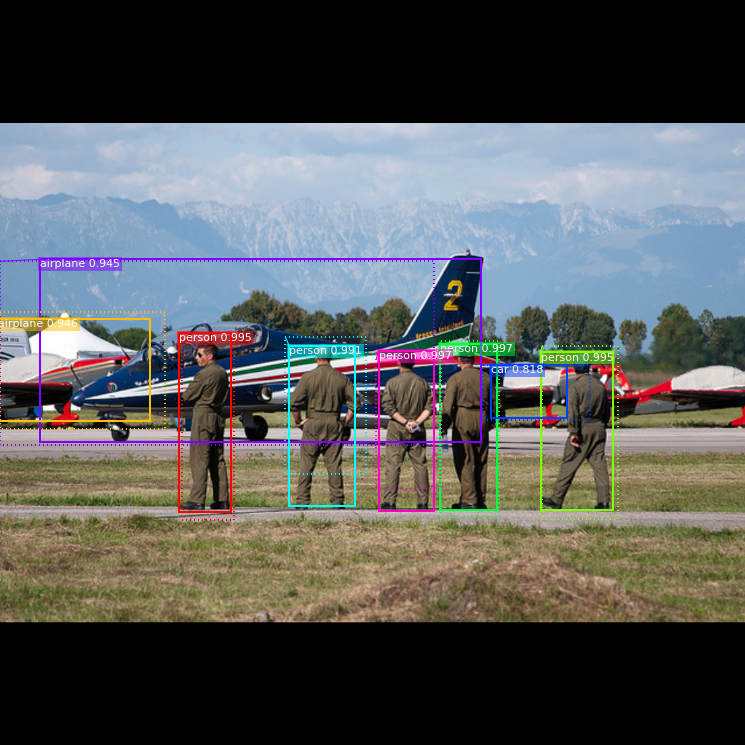
\includegraphics[scale=0.2]{mask_results}
\end{frame}

\begin{frame}
  \frametitle{\tl{Object Detectors}}
\begin{columns}
  \column{0.5\textwidth}
  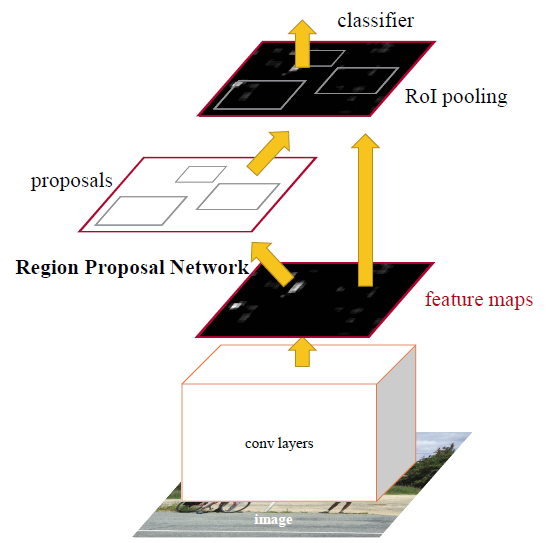
\includegraphics[scale=0.2]{fasterRCNN}
  \centering
  \\
  \tl{Faster R-CNN}

  \column{0.5\textwidth}
  \centering
  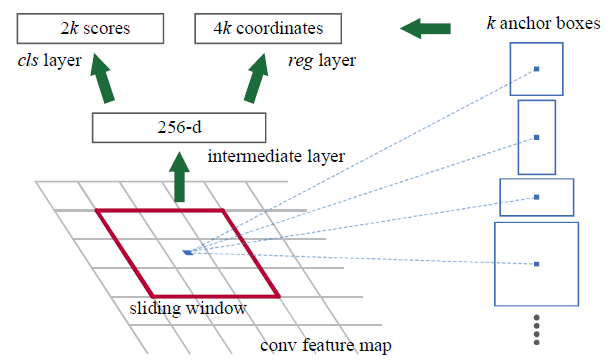
\includegraphics[scale=0.2]{rpn}
  \\
  \tl{Region Proposal \\ Network}

\end{columns}
\end{frame}


\begin{frame}
  \frametitle{\tl{Object Detectors}}
\begin{columns}
  \column{0.5\textwidth}
  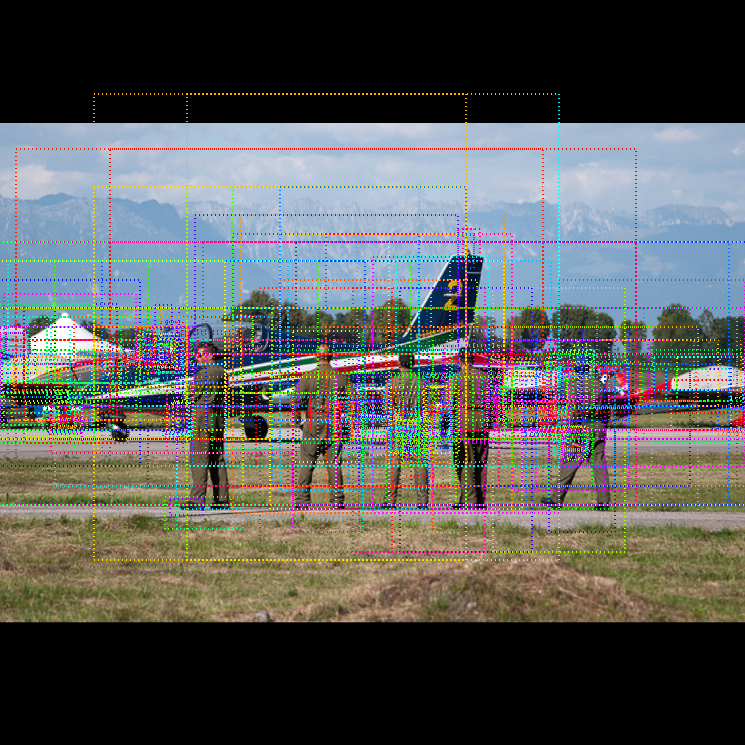
\includegraphics[scale=0.2]{mask_proposals}
  Προτάσεις περιοχών 
  \centering
  \column{0.5\textwidth}
  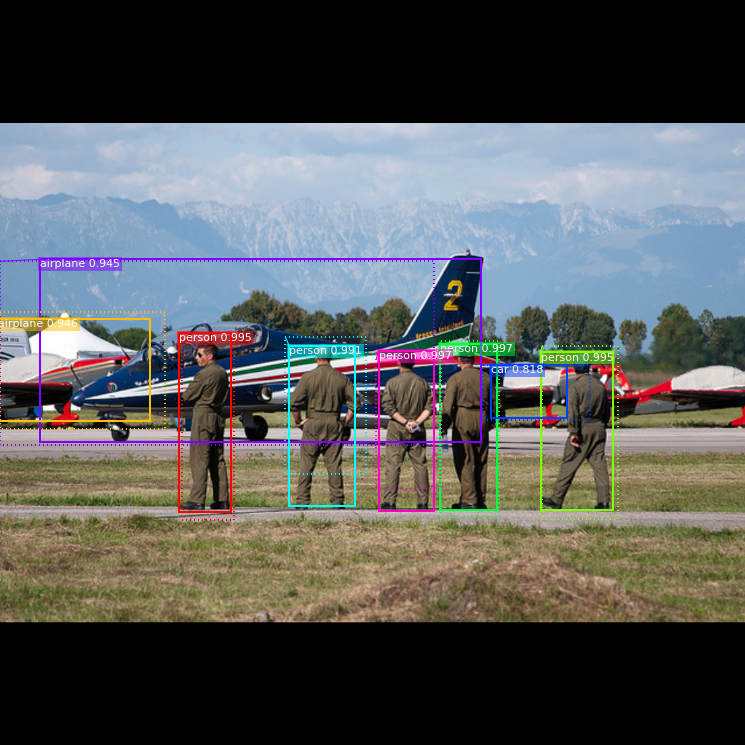
\includegraphics[scale=0.2]{mask_results}
  \centering
  Αποτελέσματα
\end{columns}
\end{frame}


\begin{center}
\begin{frame}
  \frametitle{\tl{Losses}}
\end{frame}
\begin{frame}
\begin{columns}

  \frametitle{\tl{Metrics}}
  \column{0.3\textwidth}
  \tl{Mean Average Best Overlap \\(MABO)} \\
  \column{0.7\textwidth}
  \begin{tikzpicture}
    \node (img1) {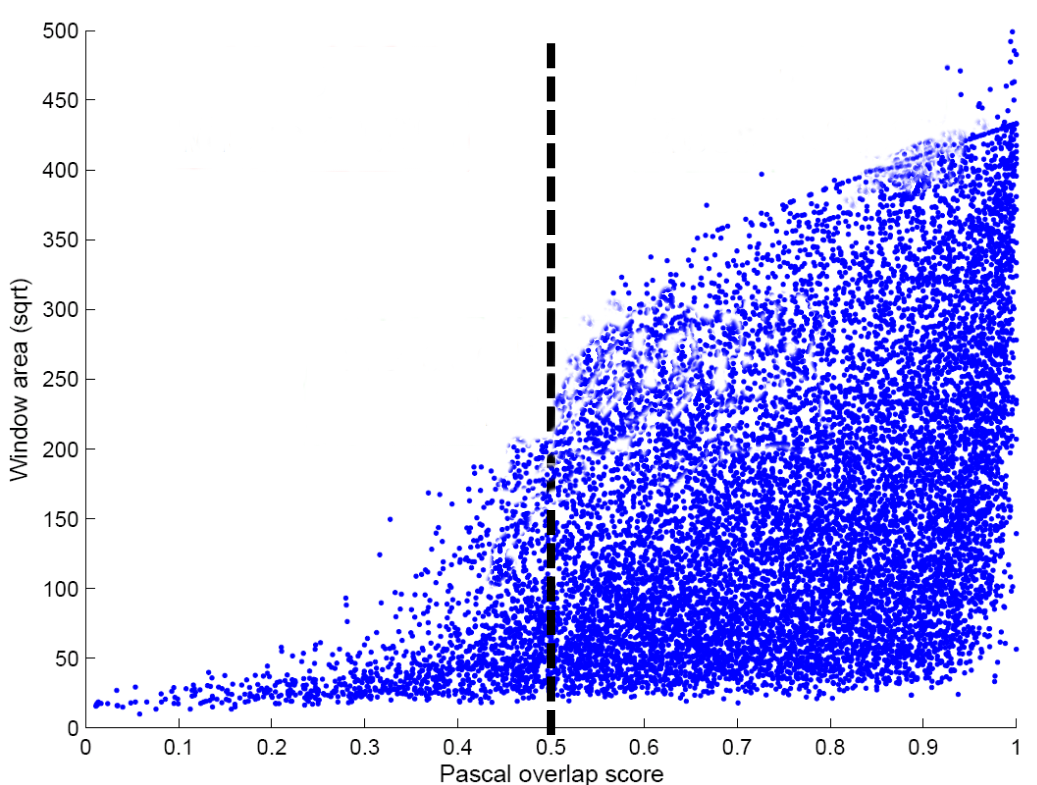
\includegraphics[height=5cm]{maboorig_01}};
    \pause
    \node (img2) at (img1.center) {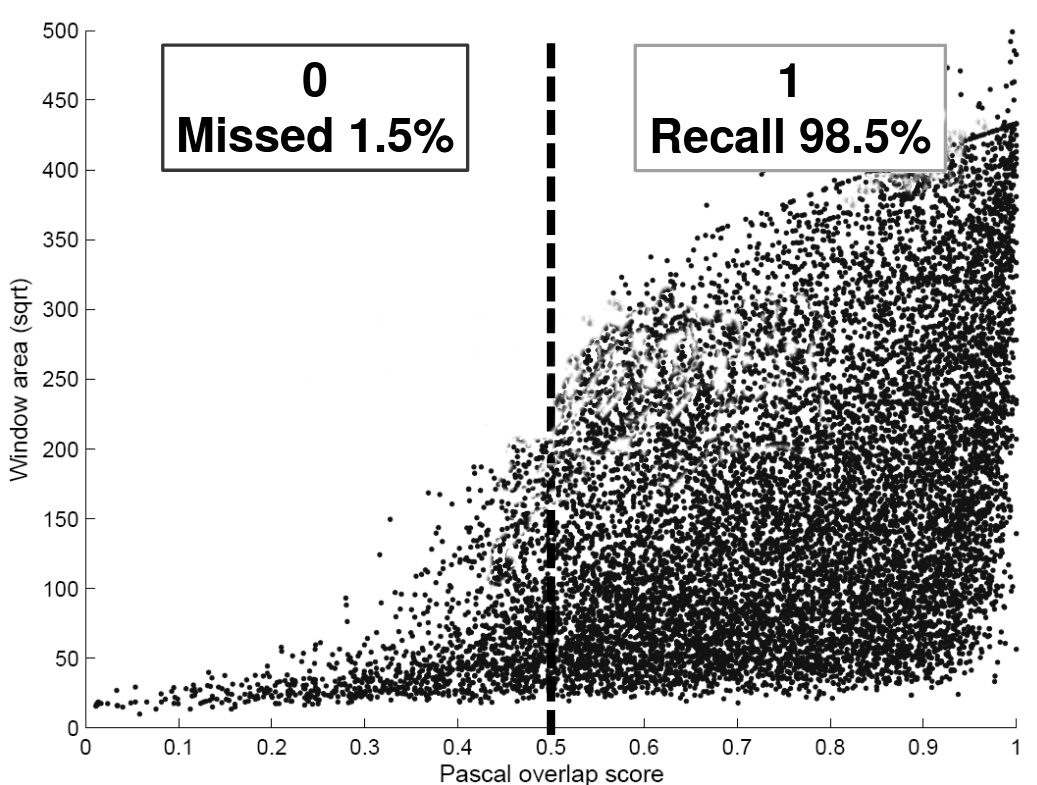
\includegraphics[height=5cm]{maboorig_02}};
    \pause
    \node (img3) at (img2.center) {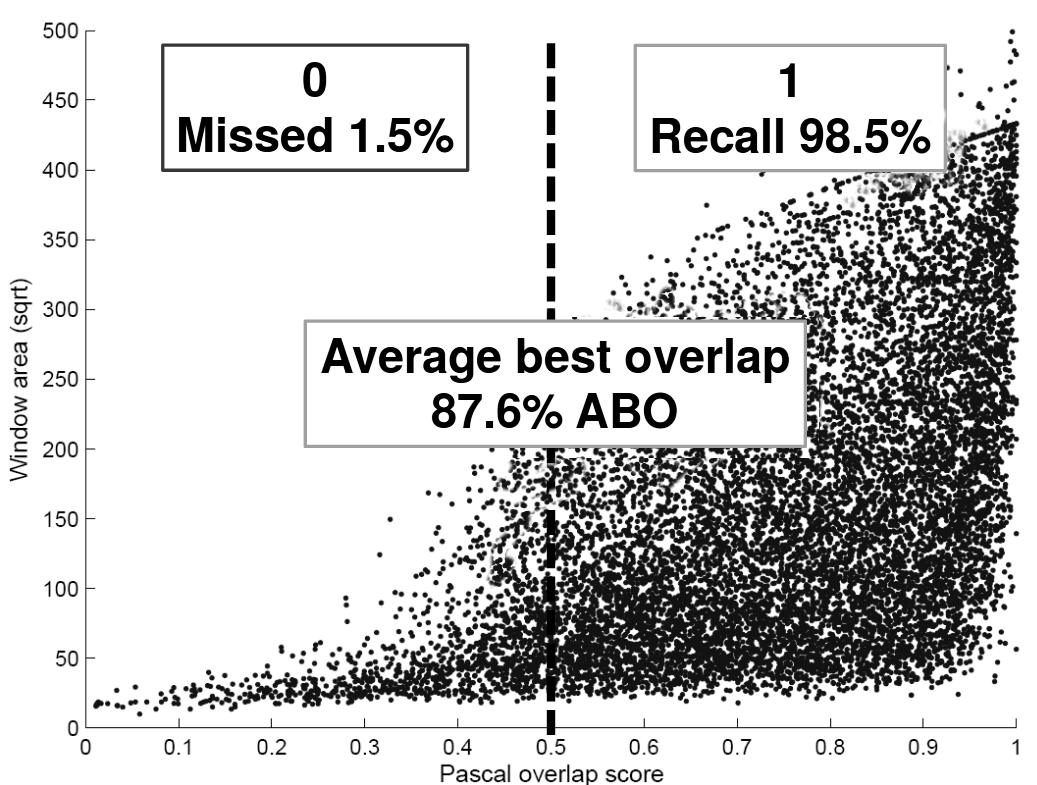
\includegraphics[height=5cm]{maboorig_03}};
  \end{tikzpicture}

\end{columns}  
\end{frame}
\end{center}

\subsection{1\textsuperscript{η} προσέγγιση}
\begin{frame}
  \frametitle{Αρχική προσέγγιση}
  
  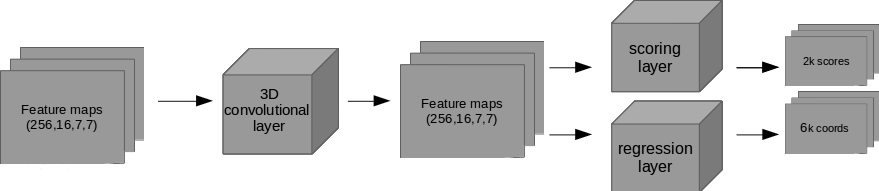
\includegraphics[scale=0.3]{tpn_1_1}

  \begin{itemize}
  \item 1 \tl{3D Convolutional Layer} με  \tl{kernel size = 3, \\
      stride = 3} και \tl{padding = 1}
  \item 1 \tl{Classification Layer}
  \item 1 \tl{Regression Layer} 
  \end{itemize}
\end{frame}

\begin{frame}
  \centering
  \frametitle{Βελτίωση της μεθόδου}
  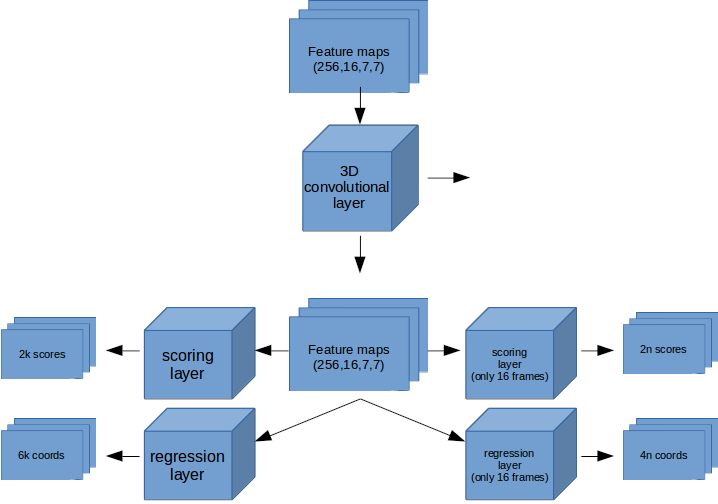
\includegraphics[scale=0.3]{tpn_1_2}
\end{frame}

\begin{frame}
  \frametitle{Βελτίωση της μεθόδου}
  \begin{columns}
  \column{0.4\textwidth}
  \centering
  \begin{itemize}
  \item 1 \tl{3D Convolutional Layer} με  \tl{kernel size = 3, \\
      stride = 3} και \tl{padding = 1}
  \item 2 \tl{Classification Layer}
  \item 2 \tl{Regression Layer} 
  \end{itemize}

  \column{0.6\textwidth}
  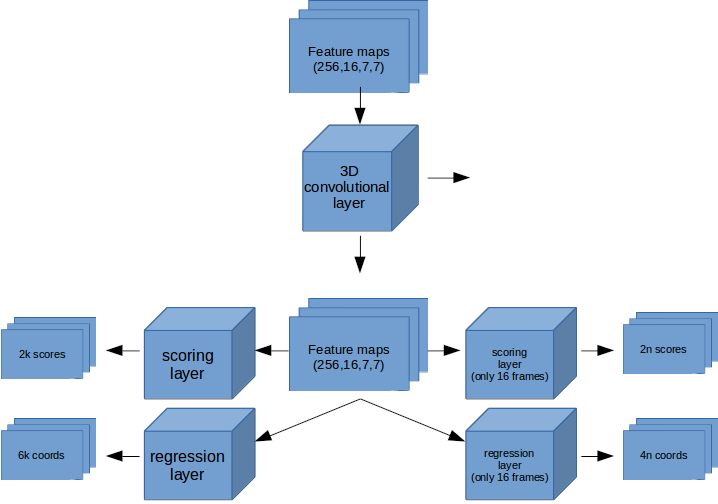
\includegraphics[scale=0.25]{tpn_1_2}
  \end{columns}
\end{frame}

\subsection{2\textsuperscript{η} προσέγγιση}

\begin{frame}
\frametitle{2\textsuperscript{η} προσέγγιση}
  \centering
  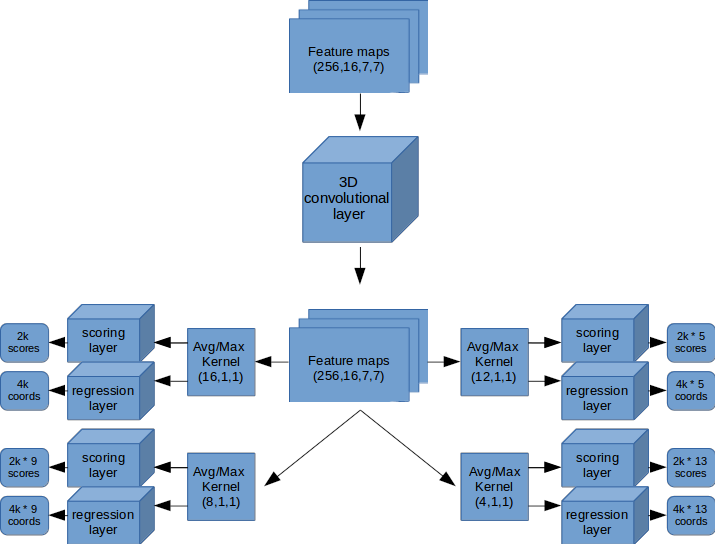
\includegraphics[scale=0.28]{tpn_2}
\end{frame}

\begin{frame}
\frametitle{2\textsuperscript{η} προσέγγιση}
  \begin{columns}
  \column{0.4\textwidth}

  \begin{itemize}
  \item 1 \tl{3D Convolutional Layer} με  \tl{kernel size = 3, \\
      stride = 3} και \tl{padding = 1}
  \item  4 \tl{Max Pooling Layers} \\
  \item 4 \tl{Classification Layer}
  \item 4 \tl{Regression Layer} 
  \end{itemize}

  \column{0.6\textwidth}
  \centering
  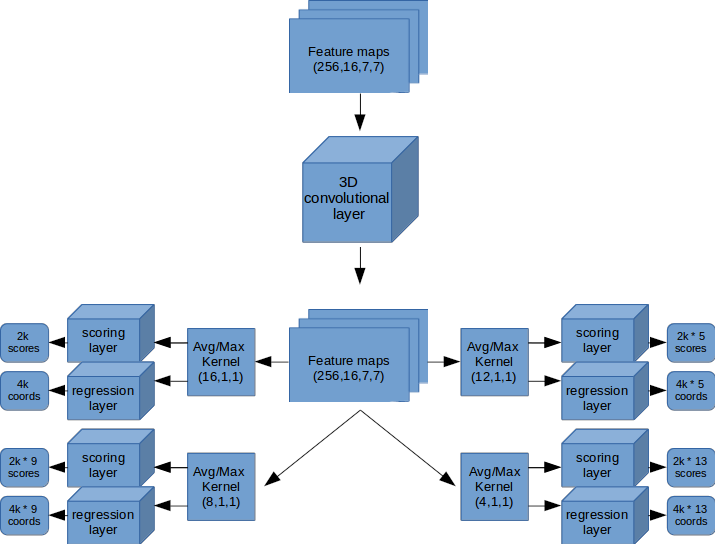
\includegraphics[scale=0.28]{tpn_2}
  \end{columns}
\end{frame}

% \end{document}